\documentclass[11pt,a4paper]{article}
\usepackage{booktabs}
\usepackage{caption}  
\usepackage{changepage}
\usepackage{geometry}
 \usepackage{pgfplots}
 \usepgfplotslibrary{dateplot}
\usepackage{diagbox}
\usepackage{tcolorbox}
\usepackage{xpinyin}
\usepackage{subfigure}
\usepackage{float}
\usepackage{multicol}
\usepackage{multirow}
\usepackage[T1]{fontenc}
\usepackage[utf8]{inputenc}
\usepackage{authblk}
\usepackage{threeparttable}
\usepackage{amsmath}

\geometry{top=1.5cm,bottom=1.5cm,left=1.5cm,right=1.5cm}

\title{Math 286 Lab Project}
\date{2020, Sept, 11th}
\author{\textbf{Ruan Yucheng} 3180111}
\author{\textbf{Zhang Zheyuan} 3180111607}
\author{\textbf{Wu Zheyu} 3180111}
\author{\textbf{Qian Chen} 3180111591}
\author{\textbf{Zheng Xiuwen} 3180111}
\affil{Department of Mechanical Engineering, ZJUI}
\renewcommand\Authands{ and }

\begin{document}
\maketitle

\section{Problem 1}
Determine the maximal solution of the following ODE with the initial value.
\begin{equation}
	y' = t^2+y^3, y(0)=1	\tag{IVP1}  \label{IVP1}
\end{equation}
\subsection{Direction Field}
At first, we plot the direction field of (1). After connecting the direction arrows we find that the curve seems has 2 vertical asymptotes, which approximately lies between -2.1 to -2.2 and 0.8 to 0.9.

\begin{center}
	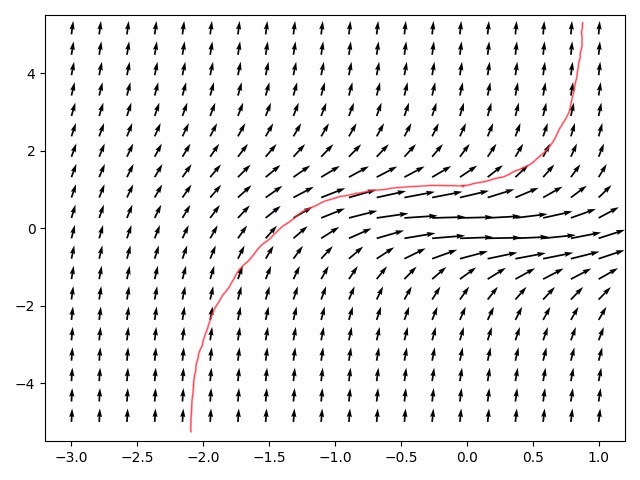
\includegraphics[scale=0.3]{HandSketch.jpeg}
\end{center}

\subsection{Numerical Methods}

\subsubsection{Methods}
\begin{table}[H]
	\begin{center}
		\scriptsize
		\renewcommand{\arraystretch}{1.3} % default is 1.0
		\begin{tabular}{p{8cm}|p{8cm}}
			\textbf{Euler}: <code>			& \quad\textbf{Heun}: <code>				\\
			$y_{n+1} = y_n+h \cdot f(t_n, y_n)$	& \quad$ k_{1,n} = f(t_n,y_n)$				\\
			$ t_{n+1} = t_n+h$				& \quad$ k_{2,n} = f(t_n+h, y_n+h \cdot k_{1,n})$	\\
											& \quad$ y_{n+1} = y_n+h \cdot f(t_n, y_n)$		\\
											& \quad$ t_{n+1} = t_n+h$					\\
										 	
			
			\textbf{Runge Kutta}: <code>										&					\\
			$ k_{1,n} = f(t_n,y_n)$												&					\\
			$ k_{2,n} = f(t_n+\frac{h}{2}, y_n+\frac{h}{2} \cdot k_{1,n})$			&					\\
			$ k_{3,n} = f(t_n+\frac{h}{2}, y_n+\frac{h}{2} \cdot k_{2,n})$			&					\\
			$ k_{4,n} = f(t_n+h, y_n+h \cdot k_{3,n})$								&					\\
			$ y_{n+1} = y_n+\frac{h}{6} \cdot (k_{1,n}+2 \cdot (k_{2,n}+k_{3,n})+k_{4,n})$	&					\\
			$ t_{n+1} = t_n+h$													&					\\
			
		\end{tabular}
	\end{center}
\end{table}

\subsubsection{Approximation}
\noindent We apply three methods all together with a step of $h = 0.1$ obtain the table below:
\begin{table}[H]
	\begin{center}
		\scriptsize
		\renewcommand{\arraystretch}{1.2} % default is 1.0
		\begin{tabular}{l|r|r|r|r|r|r|r|r}
			\textbf{T}	&\textbf{-2.3}	&\textbf{-2.2}	&\textbf{-2.1}	&\textbf{-2.0}	&\textbf{0.7}	&\textbf{0.8}	&\textbf{0.9}	&\textbf{1.0}	\\
			\hline
			Euler		&-19.87			&-9.10			&-5.05			&-3.08			&3.41			&4.85			&7.66			&14.31			\\	
			\hline
			Heun		&-5.48E5		&-175.74		&-17.44			&-6.25			&5.36			&11.14			&48.95			&4479.18		\\
			\hline
			RK			&-1.62E99		&-2.59E7		&-36.57			&-7.12			&5.89			&16.04			&2777.84		&5.43E35		\\
		\end{tabular}
	\end{center}
\end{table}

Combined with the table, the direction field and the hand-drawing sketches, we could find that the results diverses dramatically large around -2.2 to -2.1 and 0.8 to 0.9. Which may conform with our initial observation. To verify this we apply three methods altogether with smaller steps at these points.

\begin{table}[H]
	\scriptsize
	
	\begin{center}
		\begin{threeparttable}
			\renewcommand{\arraystretch}{1.2} % default is 1.0
			\begin{tabular}{r|r|r|r|r|r|r|r|r|r|r|r|r}
				\multirow{2}*{\diagbox{h}{t}}&\multicolumn{3}{c|}{-2.2} &\multicolumn{3}{c|}{-2.1}&\multicolumn{3}{c|}{0.8}&\multicolumn{3}{c}{0.9} \\
				\cline{2-13}
						&Euler	&Heun			&RK		&Euler	&Heun	&RK		&Euler	&Heun	&RK		&Euler	&Heun	&RK		\\
				\hline
				0.05 	&-12.20	&-151.20		&-1.22E5&-5.61	&-11.55	&-13.01	&5.16	&8.23	&8.77	&9.27	&34.28	&81.49	\\
				0.01 	&-1.43E5&-inf\tnote{*}	&-inf	&-16.81	&-30.33	&-31.53	&10.67	&13.98	&14.10	&103.56	&5.96E26&inf	\\
				0.001	&-inf	&-inf			&-inf	&-38.88	&-45.05	&-45.09	&15.60	&16.28	&16.28	&inf	&inf	&inf	\\
				0.0001	&-inf	&-inf			&-inf	&-46.29	&-47.10	&-47.10	&16.46	&16.54	&16.55	&inf	&inf	&inf
			\end{tabular}
			\begin{tablenotes}
				\footnotesize
				\item[*] inf stands that the calculated result is larger than the largest number that can be hold by numpy.
			\end{tablenotes}
			\setlength{\abovecaptionskip}{0.1cm}
			\setlength{\belowcaptionskip}{-0.9cm}
			\caption{Calculated Results in Different $h$}\label{tab:tab1.2.2.1}
		\end{threeparttable}
		
	\end{center}
\end{table}
From Table \ref{tab:tab1.2.2.1} we could find that $y$ at $t = -2.2$ and $t = 0.9$ if we decrease the step size, the value will increase/decrease rapidly and finally exceed the range that numpy can hold. But when $t = -2.1$ and $t = 0.8$, $y$ will finally get to a certain value.

The large difference among the computed values with different step size at $t = -2.2$ and $t = 0.9$ indicated that there may has 2 vertical asymptotes lies in $-2.2<t<2.1$ and $0.8<t<0.9$, respectively. To narrow down the interval, we chose fourth order  Runge-Kutta method with a smaller step size $h=0.0000001$. In comparision, we also compute the Improved Euler (Heun) Method's results.

\begin{table}[H]
	\scriptsize
	
	\begin{center}
		\renewcommand{\arraystretch}{1.2} % default is 1.0
		\begin{tabular}{l|r|r|r|r|r|r|r}
			\textbf{T}	&\textbf{-2.1206582}	&\textbf{-2.1206583}	&\textbf{-2.1206584}	&\textbf{-2.1206585}		&\textbf{-2.1206586}	&\textbf{-2.1206587}	&\textbf{-2.1206588}	\\
			\hline
			Heun		&-3354392.36			&-4920325.98			&-8825532.00			&-26522181.22				&-530832939.07			&-4.12E+33				&-1.44E+33				\\
			\hline
			RK			&-3520929.53			&-5430876.24			&-11766978.25			&-211743592.76				&-1.37E+24				&-6.39E+276				&-inf					\\
		\end{tabular}
		\setlength{\abovecaptionskip}{0.1cm}
		\setlength{\belowcaptionskip}{-0.9cm}
		\caption{Runge Kutta and Heun Results with $h=0.0000001$ around -2.1}\label{tab:tab1.2.2.2}
	\end{center}
	
\end{table}

\begin{table}[H]
	\scriptsize
	
	\begin{center}
		\renewcommand{\arraystretch}{1.2} % default is 1.0
		\begin{tabular}{l|r|r|r|r|r|r}
			\textbf{T}	&\textbf{0.8588757}	&\textbf{0.8588758}	&\textbf{0.8588759}	&\textbf{0.8588760}		&\textbf{0.8588761}	&\textbf{0.8588762}	\\
			\hline
			Heun		&3478801.43			&5183244.40			&9623270.74			&32083922.20			&995096229.24		&500217988540590.00	\\
			\hline
			RK			&3664014.20			&5778202.21			&13477433.90		&537639394.88			&2.66E+30			&inf				\\
		\end{tabular}
		\setlength{\abovecaptionskip}{0.1cm}
		\setlength{\belowcaptionskip}{-0.9cm}
		\caption{Runge Kutta and Heun Results with $h=0.0000001$ around 0.8}\label{tab:tab1.2.2.3}
	\end{center}
	
\end{table}
From Table \ref{tab:tab1.2.2.2} and Table \ref{tab:tab1.2.2.3} we could find there two abrupt increments, which are located at around -2.1206585 to -2.1206586 and 0.8588759 to 0.8588761, respectively. Based on this we could obtain two asymptotes with 6 digit accuracy, which are -2.120659 and 0.858876. In other words, the domain of \ref{IVP1} is $(-2.120659, 0.858876)$.

\subsection{Analytical Methods}
\subsubsection{Power Series}
\begin{table}[H]
	\scriptsize
	\begin{center}
		\renewcommand{\arraystretch}{2} % default is 1.0
		\begin{tabular}{p{10cm}|p{10cm}}
			$y = \sum_{n=0}^{\infty}a_n \cdot t^n$									&\quad$n=0, a_1=a_0^2$\\
			$y'= \sum_{n=0}^{\infty}a_{n+1} \cdot t^n$								&\quad$n=1, 2 \cdot a_2=2 \cdot a_0 \cdot a_1+a_0$\\
			$t \cdot y = \sum_{n=0}^{\infty}a_n \cdot t^{n+1}$								&\quad$n=2, 3 \cdot a_3=1+a_1^2+2 \cdot a_0 \cdot a_2$\\
			$t^2=\sum_{n=0}^{\infty}(\sum_{k=0}^{\infty} \cdot a_k \cdot a_{n-k}) \cdot t^n$		&\quad$n\geq3, (n+1) \cdot a_{n+1}=\sum_{k=0}^{n} \cdot a_k \cdot a_{n-k}+a_{n-1}$\\
			$t^2+y^2+t \cdot y=t^2+\sum_{n=0}^{\infty}(\sum_{k=0}^{\infty} \cdot a_k \cdot a_{n-k}) \cdot t^n+\sum_{n=0}^{\infty} \cdot a_n \cdot t^{n+1}$
		\end{tabular}
	\end{center}
\end{table}

As we know $y(0)=1$, applying $a_0=1$ to the recursion formula we could obtain a equation that can be easily to calculate:
\begin{center}
	$y=1+x+1.5 \cdot x^2+2 \cdot x^3+2.125 \cdot x^4+2.5 \cdot x^5+2.8958 \cdot x^6+...$
\end{center}

In our code we could modify the number of terms based on the accuracy we need. <code>

\subsubsection{Analytical Method for Vertical Asymptotes}

\begin{multicols}{2}
	\small
	\paragraph{\small Analytical Method on the Right}
	
	~\\
	
	\noindent Note that, on $0\leq t \leq 1$,

	\begin{center}
		$y'=y^2+t \cdot y+t^2 \geq t \cdot y$

		therefore $y \geq e^{\frac{t^2}{2}}>0$
	\end{center}

	\noindent Note that we have ensure that the vertical asymptote locates in the interval $0.8\leq t \leq 0.9$ from the direction field. Based on this, we could have a further squeeze formula: 
	\begin{center}
		$y^2+0.8 \cdot y+0.8^2 \leq y' = y^2+t \cdot y+t^2 \leq y^2+0.9 \cdot y+0.9^2$
	\end{center}
	\noindent Therefore, we could get the lower bound and upper bound of vertical asymptote. Considering $y_1'=y_1^2+0.9 \cdot y_1+0.9^2$ first:

	\noindent We are able to obtain th solution:
	\begin{center}
		$y_1=0.45 \cdot (\sqrt3tan(0.45 \cdot (100 \cdot sqrt3 \cdot C_1+\sqrt{3} \cdot t))-1)$
	\end{center}
	\noindent Instead of using the initial value $y(0)=1$, we use $y(0.8)=16.56526818$ which is obtained by power series to get a more accurate approximation of the vertical asymptote. Then we obtain: 
	\begin{center}
		$C_1=0.0115662936$.
	\end{center}
	\noindent We are interested in the points when $y_1 \rightarrow \infty$:
	\begin{center}
		Let $0.45 \cdot (100 \cdot \sqrt3 \cdot C_1+\sqrt3 \cdot t)=\frac{\pi}{2}$ 
		
		$\Rightarrow t_1 = 0.85873$
	\end{center}

	\noindent We could calculate in the same method on $y_2^2+0.8 \cdot y_2+0.8^2$ and obtained the solution:

	\begin{center}
		$y_2=0.4 \cdot (\sqrt{3} \cdot tan(0.4 \cdot (24 \cdot \sqrt{3} \cdot C_2+\sqrt{3} \cdot t))-1)$
	\end{center}

	\noindent Apply the initial value $y(0.8) = 16.56526818$, we get 

	\begin{center}
		$C_2=0.056333519$
	\end{center}

	\noindent When $y_2 \rightarrow \infty$, we finally get $t_2=0.85891$

	\noindent Therefore, we conclude that the vertical asymptote on the right is within the interval:
	\begin{center}
		$0.85873 \leq t \leq 0.85891$,
	\end{center}
	\noindent Which agrees with our results in numerical method well.

	\vfill\null
	\columnbreak

	\paragraph{\small Analytical Method on the Left} 

	~\\
	
	\noindent Note that, on $t \leq 0$,

	\begin{center}
		$y'=y^2+t \cdot y+t^2 \geq t \cdot y$

		therefore $y \leq -e^{-\frac{t^2}{2}} \leq 0$
	\end{center}
	\noindent Which indicates that $y' > 0$ when $t \leq 0$, so we could conclude that $y$ behaves monotonic increasing when $t \leq 0$. Therefore $y < 0$ when $t \leq 0$.

	\noindent Note that we have ensure that the vertical asymptote locates in the interval $-2.5 \leq t \leq -2$ from the direction field. Consider function $\varphi(t,y) = t \cdot y+t^2$, seeing $y$ as a constant coefficient. The axi of symmetry of the function locate $t=-\frac{y}{2}$, seeing $y$ as a constant coefficient. The axis of symmetry of the function locate $t= - \frac{y}{2}$, remembering $y<0$ when $t \leq 0$

	\noindent Based on this, we could have a further squeeze formula when $-2.5 \leq t \leq -2$

	\begin{center}
		$y^2-2 \cdot y+(-2)^2 \leq y' = y^2 + t \cdot y + t^2 \leq y^2 - 2.5 \cdot y + (-2.5)^2$
	\end{center}

	\noindent Therefore, we could get the lower bound and upper bound of vertical asymptote.

	\noindent Considering $y_1'=y_1^2-2 \cdot y_1+(-2)^2$ first:

	\noindent We are able to obtain the solution: 
	
	\begin{center}
		$y_1=\sqrt{3}tan({\sqrt{3} \cdot C_1+\sqrt{3} \cdot t})+1$
	\end{center}

	\noindent Instead of using the initial value $y(0)=1$ , we use $y(-2)=-7.1421908$ which is obtained by Runge-kutta to get a more accurate approximation of the vertical asymptote. Then we obtain: 
	
	\begin{center}
		$C_1=1.214113538$
	\end{center}

	\noindent We are interested in the points when $y_1 \rightarrow -\infty$:

	\begin{center}
		Let $\sqrt{3} \cdot C_1+\sqrt{3} \cdot t=\frac{\pi}{2}$

		$\Rightarrow t_1 = 2.1210$
	\end{center}

	\noindent We could calculate in the same method on $y_2' = y_2 ^ 2-2.5 \cdot y_2+(-2.5)^2$ and obtain the solution:

	\begin{center}
		$y_2=\frac{5}{4} \cdot (\sqrt{3} \cdot tan(\frac{5}{4} \cdot (4 \cdot \sqrt{3} \cdot C_2+\sqrt{3} \cdot t))+1)$
	\end{center}

	\noindent Apply the initial value $y(-2) = -7.1421908$, we get 
	\begin{center}
		$C_2 = 0.3477739645$
	\end{center}

	\noindent When $y_2 \rightarrow -\infty$, we finally get $t_2=-2.1166$

	\noindent Therefore, we conclude that the vertical asymptote on the right is within the interval:

	\begin{center}
		$-2.1210 \leq t \leq -2.1166$
	\end{center}

	\noindent Which conforms our result in numerical approximation well.

\end{multicols}

\newpage
\subsection{Conclusion}

\subsubsection{Error Comparison}
 
\indent We treat the value calculated by power series at t = 0.8 (within 4000 terms) as the 'exact value'. Based on this we started our error analysis. Table \ref{tab:tab1.4.1.1} shows the values calculated by three numerical methods at t=0.8 and their error compared with the 'exact value'.We could find that in this problem, if we take the same step size, Runge-Kutta method and Improved Euler method performs better in terms of accuracy.
\begin{table}[H]
	\begin{center}
		\small
		\begin{tabular}{r|r|r|r|r|r|r}
			\renewcommand{\multirowsetup}{\centering}
			exact value:&\multirow{2}*{ Euler}&\multirow{2}*{ Euler Error}&\multirow{2}*{ Heun}&\multirow{2}*{ Heun Error}&\multirow{2}*{ Runge-Kutta}&\multirow{2}*{ RK Error}\\
			 16.565268184&&&&&&\\
			 \hline
			h = 0.01		&10.67203515	&-35.5758\%		&13.9787667		&-15.6140\%	&14.10105738	&-14.8758\%	\\
			h = 0.001		&15.60414001	&-5.8021\%		&16.27971628	&-1.7238\%	&16.28178618	&-1.7113\%	\\
			h = 0.0001		&16.46233358	&-0.6214\%		&16.53646519	&-0.1739\%	&16.53648707	&-0.1737\%	\\
			h = 0.00001		&16.55490058	&-0.0626\%		&16.56238545	&-0.0174\%	&16.56238567	&-0.0174\%	\\
			h = 0.000001	&16.56451894	&-0.0045\%		&16.56526818	&0.0000\%	&16.56526818	&0.0000\%	\\
			h = 0.0000001	&16.56519326	&-0.0005\%		&16.56526818	&0.0000\%	&16.56526818	&0.0000\%	\\
		\end{tabular}
		\setlength{\abovecaptionskip}{0.1cm}
		\setlength{\belowcaptionskip}{-0.9cm}
		\caption{Error Analysis} \label{tab:tab1.4.1.1}
	\end{center}
\end{table}

\subsubsection{Conclusion}

In this problem we try to solve the IVP $y'=y^2+t \cdot y+t^2, y(0)=1$ with three numerical method: Euler Method, Heun Method and Runge-Kutta Method. In the last section we calculated the error at $t = 0.8$ of three methods with different steps and we could find that, Runge-Kutta achieves highest accuracy under same step size. In this problem The Heun method also achieves good accuracy. But the accuracy comes with price. While calculating we found that Euler Method is faster than the other two methods. The gap is widened when smaller step was applied. We recorded the time each method spent under the condition that $h=0.0000001$ and found that the Heun Method spent about 1 time longer than Euler, while Runge-Kutta roughly spent 3 times longer.

\begin{table}[H]
	\begin{center}
		\small
		\begin{tabular}{c|c|c}
			\renewcommand{\multirowsetup}{\centering}
			Euler			&Heun			&Runge Kutta	\\
			\hline
			8.82 sec		&18.71 sec		&41.04 sec		\\
		\end{tabular}
		\setlength{\abovecaptionskip}{0.1cm}
		\setlength{\belowcaptionskip}{-0.9cm}
		\caption{Time Spent to Calculate $y(0.8), h = 0.0000001$} \label{tab:tab1.4.2.1}
	\end{center}
\end{table}

During our calculation, we find that the values closed to the asymptotes are more than tricky. Therefore, to determine the more accurate locations of asymptotes and verify our numerical methods, squeeze rule has been used. Figure \ref{fig:1.4.2.1} is the plot based on Runge-Kutta method with step size 0.0000001.

\begin{center}
	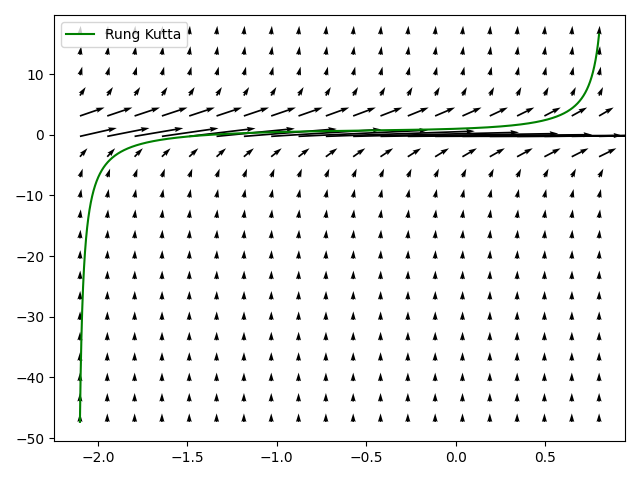
\includegraphics[scale=0.3]{P1FinalSolution.png}\label{fig:1.4.2.1}
\end{center}

\section{Problem2}

Determine the maximal solution of the following ODE with the initial value.

\begin{equation}
	y' = y^3+t \cdot y^3 + t^2 \cdot y + t^3, y(0)=1 \tag{IVP2} \label{IVP2}
\end{equation}

\subsection{Direction Field}

First First, we draw the direction field of \ref{IVP2}. We can infer from the figure that the solution to problem 2 with initial value $y(0) = 1$ has a right vertical asymptote between 0.4 and 0.6. Besides, it seems that the solution has a left slanted asymptote.

\subsection{Numerical Analysis}

To verify this observation, we first apply the Euler method and Improved Euler Method with different step sizes to approximate the right vertical asymptote at t=0.4 and t=0.5. The results are as follows:

\begin{table}[H]
	\begin{center}
		\scriptsize
		\renewcommand{\arraystretch}{1.2}
		\begin{tabular}{c|r|r|r|r}
			\multirow{2}*{\diagbox{h}{t}}&\multicolumn{2}{c|}{0.4}&\multicolumn{2}{c}{0.5}\\
			\cline{2-5}&Euler&Heun&Euler&Heun\\
			\hline
			0.1&1.4769&1.7128&1.8805&2.7722\\
			0.05&1.8161&2.1699&2.8257&7.02571\\
			0.01&2.6593&3.0070&756.8174&inf\\
		\end{tabular}
			\setlength{\abovecaptionskip}{0.1cm}
		\setlength{\belowcaptionskip}{-0.9cm}
		\caption{Euler and Heun Approximation at t = 0.4 \& 0.5 within different steps}\label{tab:tab2.2.1}
	\end{center}
\end{table}

The large difference among the computed values at t=0.5 suggests that the right vertical asymptote is lower that 0.5. Therefore, we tried several times to narrow down the interval and use the more accurate method Runge-Kutta method with fourth-order four-stage to approximate the value of the solution at $t=0.439$ and $t=0.440$.

\begin{table}[H]
	\begin{center}
		\scriptsize
		\renewcommand{\arraystretch}{1.2}
		\begin{tabular}{l|l|l}
			step h  & t=0.439 & t=0.440  \\
			\hline
			0.0005  & 18.7523 & 35.1483  \\
			\hline
			0.0001  & 22.2170 & 249.3580 \\
			\hline
			0.00001 & 23.2974 & inf     
		\end{tabular}
	\end{center}
\end{table}

\end{document}